\documentclass{article}
\usepackage{spconf,amsmath,graphicx,hyperref}
\usepackage{amsmath}
\usepackage[flushleft]{threeparttable}
\usepackage{cite}
\usepackage{booktabs, multirow}
\usepackage{enumitem} %缩进itemize
\usepackage{amssymb}

\usepackage[table]{xcolor}
\usepackage{pgf}

\definecolor{heatblue}{RGB}{65,115,200}
\definecolor{heatred}{RGB}{205,92,92}

\newcommand{\heatpos}[1]{%
  \pgfmathtruncatemacro{\shadevalue}
    {min(54,14+40*sqrt((#1)/10))}%
  \edef\heatcolor{heatblue!\shadevalue}%
  \expandafter\cellcolor\expandafter{\heatcolor}%
  $+$#1%
}

\newcommand{\heatneg}[1]{%
  \pgfmathtruncatemacro{\shadevalue}
    {min(54,14+40*sqrt((#1)/10))}%
  \edef\heatcolor{heatred!\shadevalue}%
  \expandafter\cellcolor\expandafter{\heatcolor}%
  $-$#1%
}

\newcommand{\heatposbest}[1]{%
  \pgfmathtruncatemacro{\shadevalue}
    {min(54,14+40*sqrt((#1)/10))}%
  \edef\heatcolor{heatblue!\shadevalue}%
  \expandafter\cellcolor\expandafter{\heatcolor}%
  $\mathbf{+}$\textbf{#1}%
}

\newcommand{\heatnegbest}[1]{%
  \pgfmathtruncatemacro{\shadevalue}
    {min(54,14+40*sqrt((#1)/10))}%
  \edef\heatcolor{heatred!\shadevalue}%
  \expandafter\cellcolor\expandafter{\heatcolor}%
  $\mathbf{-}$\textbf{#1}%
}

% \usepackage{lilyglyphs} % dynamic symbols
% \usepackage{tikz}
% \usetikzlibrary{arrows.meta,positioning,fit,calc}
% \tikzset{
%   block/.style={draw, rounded corners, very thick, align=center, inner sep=3pt, minimum height=8mm, fill=white},
%   tinyblock/.style={draw, rounded corners, thick, inner sep=2pt, minimum height=4mm, fill=white},
%   arrow/.style={-Latex, very thick}
% }

\title{CASM: A Context-Aware Semi-Markov Alternative to DBN Post-Processor for Beat Tracking}

\name{Zhanhong He$^{1}$, Hanyu Meng$^{2}$, Yaolong Ju$^{3}$}
\address{
    $^{1}$The University of Western Australia, Perth, Australia\\
    $^{2}$The University of New South Wales, Sydney, Australia\\
    $^{3}$Great Bay University, Guangdong, China
}

\begin{document}
\ninept
\maketitle

\begin{abstract}
The last stage of beat tracking must turn dense neural activations into a
discrete, musically coherent event sequence. Direct peak picking preserves
local evidence but can fragment the pulse, whereas dynamic Bayesian networks
(DBNs) restore continuity through globally configured tempo and meter
assumptions. PLPDP showed that these assumptions can instead be informed by
local periodicity, but a locally preferred pulse may itself be ambiguous
between competing metrical levels. Building on that insight, we introduce
CASM, a plug-in, context-aware semi-Markov decoder over a sparse graph of
activation-supported beat candidates. CASM measures the margin between the
best and competing local periods and uses it to control both the strength and
tolerance of each segment-duration potential. It commits when one pulse is
well supported and defers to the neural evidence when several interpretations
remain plausible. Beat-count and downbeat-agreement safeguards make this
behaviour deterministic and auditable. One globally calibrated configuration
is applied without backbone retraining or track-specific BPM and meter settings
to Beat This, MSCNN-lite, and TCN activations on GTZAN and SMC. The results
position CASM as a conservative F1--continuity operating point rather than a
universal replacement for DBN.
\end{abstract}

\begin{keywords}
beat tracking, downbeat, content-aware adaptation, semi-Markov decoding, post-processing, local periodicity
\end{keywords}

\section{Introduction}
\label{sec:intro}

The final decoder in a beat tracker is deceptively consequential. A neural
network can place high framewise probability on genuine beats and still leave
duplicates, gaps, metrical-level switches, or downbeats that disagree with its
beat grid. Event F-measure rewards local placement, whereas continuity metrics
also require one metrical interpretation to persist. Weak decoding therefore
respects the network but may yield an unstable clock; strong decoding restores
a clock but may overwrite correct, expressive, or unusual evidence.

A dynamic Bayesian network (DBN) addresses this problem by asking which path
through tempo, phase, and meter states best explains all frames
\cite{krebs2015dbn}. In plain terms, the input chooses a route through a
globally specified timetable: the BPM range, allowed meters, and cost of tempo
changes are fixed before the track is seen. The inferred state path is
input-dependent, but the transition law does not become softer merely because
the activation reveals a credible half- or double-tempo alternative. CASM
takes the complementary view. It considers only activation-supported peaks,
scores the complete elapsed interval between two peaks, and lets the local
activation decide how strongly regularity should count. Thus the practical
difference is not ``adaptive versus non-adaptive inference,'' but a fixed DBN
transition law versus an input-conditioned segment penalty. This distinction
matters on difficult music, where retuning a DBN can help one corpus but weakens
the claim of out-of-the-box transfer \cite{ahn2026smcblindspot}. Conversely,
post-processing-free trackers avoid some DBN errors but minimal peak picking can
sacrifice sequence continuity \cite{chen2022postprocessingfree,foscarin2024beat}.

PLPDP provides the immediate starting point for our approach. It showed that a
post-processor can replace a single global tempo preference with a local
inter-beat interval and confidence derived from predominant local pulse (PLP)
\cite{chiu2023localperiodicity}. We retain its central idea---the temporal prior
should listen to the current activation---and address a remaining risk: the
strongest local period may only narrowly beat a competing metrical level. CASM
therefore measures a best-versus-runner-up period margin. A clear winner creates
a narrow, strong duration preference; a small margin weakens and broadens it,
allowing the neural peaks to decide.

Fig.~\ref{fig:casm-examples} previews these two behaviours on real activations.
On the left, Direct retains mainly every second strong peak; CASM uses supported
local periodicity to select intervening weak maxima and repairs continuity
without moving events away from the activation. On the right, octave-related
period hypotheses compete, so CASM suppresses its structural preference and
leaves the Direct path unchanged. The latter occurs without invoking the
count-ratio safeguard: uncertainty changes the segment score itself.

\begin{figure}[t]
\centering
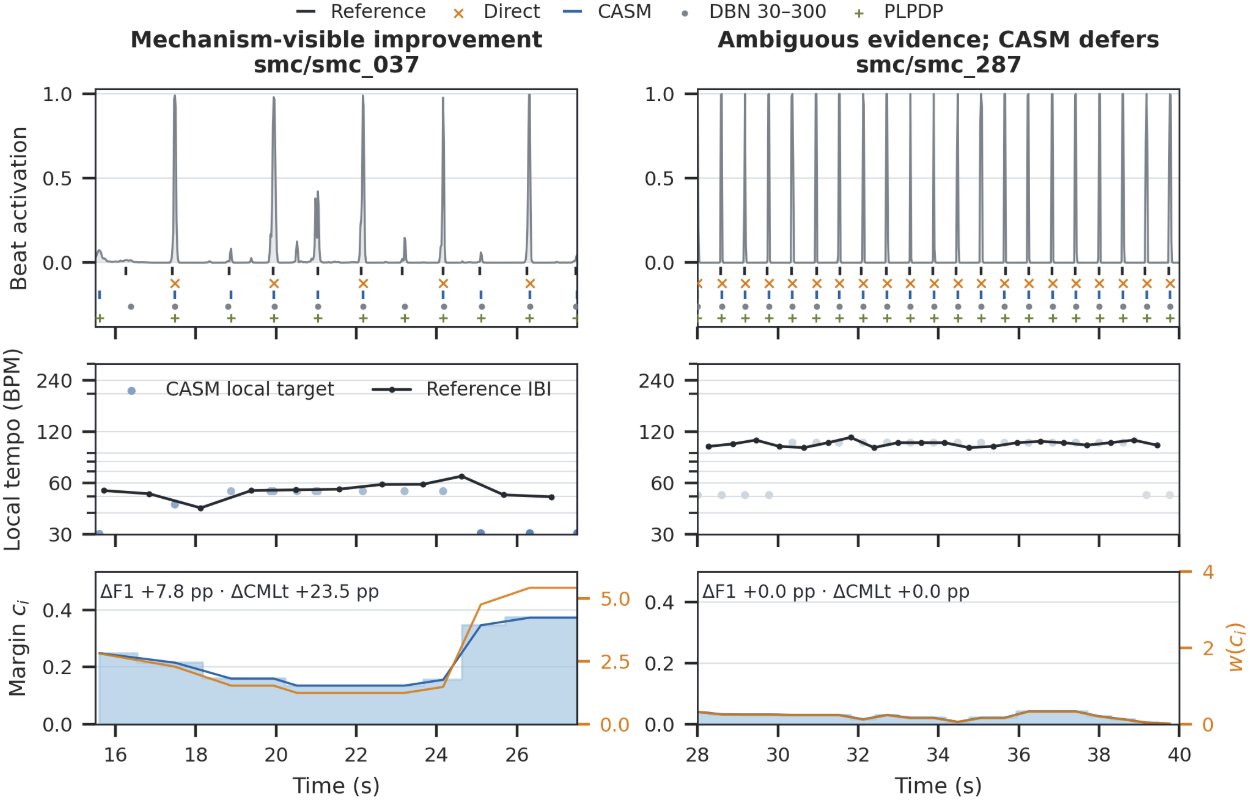
\includegraphics[width=\columnwidth]{figures/p0.jpg}
\caption{Illustrative CASM behaviour on real Beat This OOF activations from
SMC. Left: a supported local period helps recover weak, activation-supported
beats. Right: a small period margin weakens the duration term, so CASM defers
to Direct. Reference IBI is shown only for interpretation and is never observed
by CASM. Tracks and windows were selected post hoc to expose the mechanism, not
to estimate average performance.}
\label{fig:casm-examples}
\end{figure}

Our contributions are threefold:
\begin{itemize}
\item Building on PLPDP, we formulate beat decoding as a sparse semi-Markov
path whose segment target, strength, and tolerance are determined by local
period evidence and its ambiguity at both endpoints.
\item We add beat-count and downbeat-agreement safeguards to obtain a
deterministic plug-in that requires neither upstream retraining nor per-track
BPM and meter settings.
\item We study one frozen operating point across three activation backbones and
analyse how decoder-calibration scale and composition affect transfer.
\end{itemize}

\section{Related Work}
\label{sec:related}

\subsection{Structured post-processing}

Dynamic programming has long balanced onset evidence against inter-beat
regularity \cite{ellis2007beattracking}. Bayesian beat-position models used a
dominant beat interval \cite{korzeniowski2014crf}, while learned CRFs were later
extended from beats to downbeats, long-range section consistency, and
genre-specific microtiming \cite{fillon2015crf,durand2016crfdownbeat,
fuentes2019skipchain,fuentes2019microtiming}. Resonating comb filters estimate a
dominant periodicity before event alignment \cite{bock2015combfilter}, and DBNs
enumerate tempo--phase--meter states and decode their most likely trajectory
\cite{krebs2015dbn,bock2016joint}. These methods differ in state representation
and optimization, but they share a useful principle: noisy framewise evidence
should be interpreted as a sequence rather than thresholded independently.

\subsection{From PLPDP to ambiguity-aware local constraints}

PLPDP is CASM's direct methodological predecessor
\cite{chiu2023localperiodicity}. Its central diagnosis was that a fixed global
tempo penalty, including the empirically chosen transition law of common HMM
trackers, can be too rigid for expressive timing. PLPDP extracts a time-varying
inter-beat interval and a confidence curve from PLP, then replaces the global
target and weight of dense-frame dynamic programming with those local
quantities. Its real-time continuation improves controllability
\cite{meier2024realtime}, and dPLP makes local-pulse estimation differentiable
\cite{chiu2025dplp}.

CASM advances this line of work rather than treating PLPDP as an unrelated
baseline. PLPDP asks, ``What is the current local pulse, and how strong is its
PLP peak?'' CASM additionally asks, ``How decisively does that pulse beat the
next plausible explanation?'' It measures a top-versus-runner-up period margin
around each retained activation maximum, combines the two endpoint contexts,
and uses the result to change both the strength and the tolerance of a complete
event-to-event duration cost. The path is sparse and remains anchored to
observed maxima, whereas PLPDP can evaluate every frame. This extension is
designed for half/double-tempo competition: when no period wins clearly, the
decoder should not enforce any of them confidently.

Reliability-informed tracking previously established the broader principle
that temporal commitment should depend on evidence quality
\cite{degara2012reliability}. CASM's margin is a local, deterministic separation
score rather than predicted track-level accuracy. It also differs from the
causal one-dimensional semi-Markov state space of \cite{heydari2022semimarkov},
which maintains a framewise posterior and adapts a jump-back distribution
online. CASM is an offline maximum-score path over candidate-to-candidate
segments. Nor is it a semi-CRF: its potentials are hand-specified, unnormalized,
and not learned \cite{sarawagi2004semimarkov}.

\subsection{Alternatives beyond plug-in decoding}

Particle filters maintain online tempo hypotheses \cite{hainsworth2004particle},
and BeatNet/BeatNet+ extend this branch to joint real-time rhythm analysis
\cite{heydari2021beatnet,heydari2024beatnetplus}. Another line adapts a tracker
with user annotations \cite{pinto2021userdriven,maia2022adapting,
pinto2023bridging,maia2024selective,pinto2026challenging}. More recent systems
remove or redesign post-processing: masked diffusion iteratively refines
coherent sequences \cite{foscarin2026masked}, BeatFCOS predicts intervals as
objects with Soft-NMS \cite{ahn2025beatfcos}, and other work reformulates the
prediction target \cite{bolt2026reformulated}. These approaches change the
predictor or import additional supervision. CASM instead addresses the
deployment setting in which only the activation output of a frozen tracker is
available.

\section{Methodology}
\label{sec:method}

\subsection{Overview and PLPDP lineage}
\label{sec:casm}
Let a frozen tracker produce beat and downbeat logits $z_t^{\mathrm b}$ and
$z_t^{\mathrm d}$ at frame rate $F$. Like PLPDP, CASM derives a local period
and a measure of its support from the current beat activation. CASM then makes
two changes. First, it decodes only a sparse set of activation maxima rather
than every frame. Second, its support measure is the separation between the
best and competing periods, and it controls both how strongly and how narrowly
the chosen period is enforced. The global coefficients define one frozen
evidence-to-constraint rule; the input determines the operating point of that
rule at every candidate segment.

\subsection{Candidate-event segments}
Set $a_t=\operatorname{sigmoid}(z_t^{\mathrm b})$ and retain its local maxima
above threshold $\theta_{\mathrm c}$ as
$\mathcal C=\{t_1,\ldots,t_N\}$. An edge $(i,j)$ spans the complete elapsed
time $\Delta_{ij}=(t_j-t_i)/F$ and is allowed only within the 30--300 BPM
support. With $e_i$ denoting clipped activation evidence, CASM selects a path
$\pi=(i_1,\ldots,i_K)$ that maximizes
\begin{equation}
\mathcal S(\pi)=\sum_{k=1}^{K}e_{i_k}
-\sum_{k=2}^{K}D_{i_{k-1},i_k},
\label{eq:casm-objective}
\end{equation}
where $D_{ij}$ is the segment-duration cost below. This is the precise sense in
which CASM is semi-Markov: one transition consumes a variable-length
candidate-to-candidate segment and scores its duration as a whole. It is not a
generative hidden semi-Markov model, and the segment potentials are not learned.

\subsection{Local period and ambiguity}

At each candidate $i$, normalized autocorrelation scores the admissible integer
lags $\ell$ in a centred local window $\mathcal W_i$:
\begin{equation}
q_i(\ell)=
\frac{\left\langle a_u a_{u-\ell}\right\rangle_{u\in\mathcal W_i}}
{\sqrt{\left\langle a_u^2\right\rangle_{u\in\mathcal W_i}
       \left\langle a_{u-\ell}^2\right\rangle_{u\in\mathcal W_i}
       +\epsilon_q}}
\left(\frac{\ell_{\min}}{\ell}\right)^{\beta},
\label{eq:casm-local-period}
\end{equation}
with zero padding outside the signal and a mild fast-tempo prior in the final
factor. The winning lag gives $\ell_i^\star=\arg\max_\ell q_i(\ell)$ and local
period $\tau_i=\ell_i^\star/F$. We then compare it with the best lag outside a
$\pm2$-frame neighbourhood:
\begin{equation}
c_i=\operatorname{clip}_{[0,1]}\!\left(
\frac{q_i(\ell_i^\star)-
\max_{\ell:\,|\ell-\ell_i^\star|>2}q_i(\ell)}
{|q_i(\ell_i^\star)|+\epsilon_c}\right).
\label{eq:casm-reliability}
\end{equation}
Here $c_i$ is a period-separation margin, not a calibrated probability of being
correct. A large value means that one local period clearly wins; a small value
means that nearby or half/double-time explanations remain competitive. Both
$\tau_i$ and $c_i$ are median-filtered over five consecutive candidates.

\subsection{Ambiguity-conditioned segment cost}

For edge $(i,j)$, CASM symmetrizes the endpoint contexts as
$\bar\tau_{ij}=\sqrt{\tau_i\tau_j}$ and $c_{ij}=\sqrt{c_i c_j}$. Define
\begin{equation}
\begin{aligned}
\sigma(c)&=\sigma_0+(1-c)\sigma_{\mathrm u}, \\
w(c)&=\frac{\lambda c}{2\sigma(c)^2}, \\
D_{ij}&=w(c_{ij})
\left[\log\!\left(\frac{\Delta_{ij}}{\bar\tau_{ij}}\right)\right]^2.
\end{aligned}
\label{eq:casm-duration}
\end{equation}
The log ratio treats proportional timing errors symmetrically. More
importantly, the margin acts twice: high $c$ narrows $\sigma(c)$ and increases
$w(c)$, while low $c$ broadens the tolerated deviation and reduces its weight.
CASM can therefore select weak but rhythmically supported maxima when the pulse
is clear, yet avoid imposing a dubious grid when periodic evidence is
ambiguous.

Fig.~\ref{fig:casm-response} connects Eq.~\eqref{eq:casm-duration} to the
observed decoder behaviour. Panel (a) is the single response law fixed by the
global coefficients. Panel (b) shows that real edges from different backbones
and corpora occupy different parts of that law. Panel (c) aggregates the same
quantity per piece: one frozen configuration produces distinct effective
stiffness distributions, while the separately annotated fallback remains a
second safety mechanism. These panels audit input conditioning; they are not an
accuracy comparison.

\begin{figure}[t]
\centering

\includegraphics[width=\columnwidth]{figures/p1.jpg}
\caption{Input-conditioned duration stiffness under one frozen CASM
configuration. (a) The fixed constants map period margin $c$ to coefficient
$w(c)$; shading contains 99.5\% of observed structured-path edges. (b) Edge
margin distributions differ across backbones and corpora. (c) Per-piece median
coefficients therefore occupy different operating ranges; annotations give the
separate count-ratio fallback rate. Fixed parameters define one response law,
not one effective rigidity for every input.}
\label{fig:casm-response}
\end{figure}

\subsection{Decoding and safeguards}

A Viterbi-style dynamic program maximizes Eq.~\eqref{eq:casm-objective}, with a
restart option for an unfavourable prefix, and backtracks the highest-scoring
path. In parallel, we form the Direct path of \cite{foscarin2024beat} by
seven-frame max pooling, a zero-logit threshold, and one-frame deduplication.
If the structured-to-Direct event-count ratio falls outside
$[r_{\min},r_{\max}]$, CASM returns Direct. This is a deterministic sanity
check, not a learned router.

Downbeats are decoded only on the selected beat grid. A second dynamic program
links candidate downbeats separated by an allowed bar length and penalizes
unnecessary meter changes. Direct downbeat maxima are independently snapped to
the same beat grid; the meter path is retained only when it agrees sufficiently
with that snapped path, otherwise the snapped path is returned. Thus every
output downbeat remains synchronized with an output beat.

All scalar settings are calibrated once on development folds and then frozen
for every track and backbone, as detailed in Sec.~\ref{sec:exp}. CASM is
therefore input-conditioned but not parameter-free: it has no learned weights,
per-track tuning, annotated beats, BPM, or meter input at inference.


\section{Experiments}
\label{sec:exp}

\subsection{Data, backbones, and metrics}
We evaluate on GTZAN ($N=993$) using the annotations and exclusions of Beat This \cite{foscarin2024beat}, and on the deliberately difficult SMC corpus ($N=217$) \cite{smc}; SMC provides beat but not downbeat annotations. We use three 50-Hz activation backbones: the Beat This spectrogram Transformer \cite{foscarin2024beat}, the lightweight multi-scale convolutional backbone MSCNN-lite \cite{he2026dynest}, and the TCN of \cite{bock2020deconstruct}. The decoder receives only their framewise beat and downbeat logits.

For GTZAN, \texttt{final0}, \texttt{final1}, and \texttt{final2} are three independently trained full-data backbone seeds. Their training excludes GTZAN but includes SMC. We first macro-average over the same 993 tracks and then average the three seed-level scores. For SMC, using those full-data checkpoints would leak training examples; we instead use the corresponding held-out checkpoint for each of eight folds. Seven folds contain 27 tracks and the eighth contains 28; we average their fold-level macro scores. CASM itself is deterministic and has neither a neural checkpoint nor a random seed.

Following the established protocol, the first 5\,s are trimmed and \texttt{mir\_eval} computes F1 with $\pm70$\,ms tolerance, CMLt, and AMLt \cite{raffel2014mireval}. CMLt requires a continuously correct metrical level; AMLt additionally accepts the standard off-beat and half/double-level interpretations. Seed variation on GTZAN and fold variation on SMC have different replication units and are descriptive, not confidence intervals.


\subsection{Decoder baselines}
\emph{Direct} is the minimal peak picker defined in Sec.~\ref{sec:method}. \emph{DBN} is the conventional joint \texttt{madmom} configuration: meters $\{3,4\}$, 55--215 BPM, transition weight 100, observation weight 16, and threshold 0.05 \cite{krebs2015dbn}. \emph{DBN-SMC-opt} is deliberately diagnostic. Its sequential beat and bar stages were selected from 753 configurations on the TCN SMC 8-fold OOF activations, maximizing beat F1 with CMLt/AMLt tie-breaks, and only then frozen for the three backbones and GTZAN. It uses 50--215 BPM, 30 tempo states, transition/observation weights 7/20, threshold 0.3, meters $\{3,4\}$, bar-observation weight 100, and meter-switch probability $10^{-7}$. It is neither a clean SMC test nor a published SMC-specific recipe from \cite{bock2020deconstruct}.

The \emph{CRF} row uses \texttt{madmom}'s historically named \texttt{CRFBeat DetectionProcessor} \cite{korzeniowski2014crf} at 30--300 BPM with interval width 0.18; it should not be confused with the learned CRF in \cite{fillon2015crf}. \emph{CombFilter} uses \texttt{madmom}'s global tempo/iterative-alignment processor \cite{bock2015combfilter}. CRF and CombFilter decode downbeat activations at 8--100 BPM and snap their outputs to their respective beat grids.

\subsection{Frozen operating point and scale analysis}
Every CASM row in Sec.~\ref{sec:results} uses exactly one explicitly loaded
Frozen-4F configuration:
\[
\begin{split}
&F=50,\quad \theta_{\mathrm c}=0.03,\quad
(B_{\min},B_{\max})=(30,300),\\
&|\mathcal W|=8{\rm\,s},\quad \beta=0.15,\quad
(T,L)=(2,6),\\
&(\lambda,\sigma_0,\sigma_{\mathrm u})=(4,0.12,0.40),\quad
[r_{\min},r_{\max}]=[0.85,1.8],\\
&\mathcal M=\{2,\ldots,7\},\quad
(T_{\mathrm d},\eta,\rho,\gamma)=(4,3,0,0.6).
\end{split}
\]
Its scalar settings were selected on the union of SMC folds $\{2,7,1,3\}$ and then reused for all tracks and all backbones. Thus context-aware means input-conditioned inference, not test-time parameter updates: CASM has validation-selected parameters, but no annotated beat, inter-beat-interval, BPM, or meter input at inference.

The choice to foreground 4F was made \emph{after} inspecting the calibration sensitivity analysis and is therefore exploratory. The seven-fold configuration is the only comparator locked before GTZAN inspection; it differs from 4F only in $\sigma\_0=0.15$. For the scale study, SMC fold 0 ($N=27$) is never used for selection. From folds 1--7 we enumerate every 1-, 2-, and 4-fold calibration subset ($7$, $21$, and $35$ combinations) plus the seven-fold union, and evaluate all locked configurations on the same SMC fold 0 and fixed GTZAN/\texttt{final1} panel. The latter panel is test-conditioned and is used only to describe sensitivity, not to claim a held-out optimum.



% \subsection{Comparison Candidates}
% \label{ssec:candidates}
% Due to the reproduceability, we are gainting several open-availble deep-learning beat tracking model as the backbone, connecting to our proposed CASM post-processor. These models are:

% (1) Beat This \cite{foscarin2024beat}: an transformer-based model, the original code, and its open-available model checkpoint was used. We only use to do re-evaluation in this progress.\\
% (2) Multi-Scale CNN \cite{}: \\
% (3) TCN \footnote{}


% Some models are trained on different data pipeline, while still fair reserved the Ballroom, Hainsworth, SMC dataset for 8-fold cross evaluation, we only reported their paper results


% \noindent\textbf{Beat This \cite{foscarin2024beat}}
% We establish single-task baselines by adapting the multi-scale network from \cite{li2023frame}, integrating their model architecture (code publicly available) into our data handling pipeline and training an independent model for each target. The loss for each single-task network is the corresponding single term from our multi-task loss, with an empirically optimal temporal scaling factor of 5.

% \noindent\textbf{Single-task Multiscale CNN (MSCNN) \cite{he2026dynest}} We report published results from representative methods in \cite{kosta2017thesis}. This includes the Artificial Neural Networks (ANN) for dynamics, and the Pruned Exact Linear Time (PELT) algorithms for change points. These methods are tuning-intensive and non-end-to-end, so we report the literature scores rather than re-implement them.

% \noindent\textbf{TCN\cite{bock2020deconstruct} and BeatThis \cite{foscarin2024beat}} We include the time-convolutional network (TCN) original by \cite{bock2020deconstruct}, and the recent state-of-the-art transformer model, Beat This \cite{foscarin2024beat}. Both models can estimate beats and downbeats simultaneously. We retrain them from scratch on the MazurkaBL dataset using their publicly available code and the same 5-fold protocol as ours.


% \subsection{Evaluation Setup}
% \label{ssec:metrics}
% Performance on all four tasks is evaluated using the F1 score. For beat and downbeat tracking, we report F1 with a \mbox{$\pm70$\,ms} tolerance, consistent with prior work \cite{bock2020deconstruct,foscarin2024beat}. Evaluation of both dynamics and change points is consistent with \cite{kosta2017thesis}. For dynamics, the model's continuous output (dynamic level curve) is first sampled at each ground-truth beat location, and these values are then discretized into the corresponding dynamic markings. This converts the frame-wise prediction into a sequence of beat-wise labels, which are evaluated using a macro-averaged F1 score across five dynamic classes (\textit{pp, p, mf, f, ff}, excluding the \textit{blank} class). For change points, their predictions are snapped to the nearest ground-truth beat before being evaluated with a standard F1 score. This beat-wise alignment for both tasks turns the evaluation into a direct, musically metrical index-based comparison, thus requiring no additional timing tolerance.


\section{Results}
\label{sec:results}
\subsection{Main Result}


\begin{table}[t]
\centering
\caption{Comparison of beat-tracking post-processors across different backbone models. DBN default $bpm=[55,215]$ is for general music, but many SMC songs out of this range \cite{ahn2026smcblindspot}; therefore, SMC-optimized $bpm=[30,300]$ can be applied. Only BPM setups were changed in post-processors, with other default setups unchanged.}
\label{tab:postprocessor_ablation}
\begingroup
\fontsize{7.5pt}{8.5pt}\selectfont
\setlength{\tabcolsep}{0.7pt}
\renewcommand{\arraystretch}{0.92}
\resizebox{\columnwidth}{!}{%
\begin{tabular}{l|c|rrr@{\hspace{2pt}}|rrr@{\hspace{2pt}}|rrr}
\toprule
\multicolumn{1}{c|}{\multirow{2}{*}{\textbf{Method}}}
& \multicolumn{1}{c|}{\multirow{2}{*}{\textbf{BPM}}}
& \multicolumn{6}{c|}{\textbf{GTZAN (Beat / Downbeat)}}
& \multicolumn{3}{c}{\textbf{SMC (Beat)}} \\
\cmidrule(lr){3-8}
\cmidrule(l){9-11}
& & F1 & CMLt & AMLt
& F1 & CMLt & AMLt
& F1 & CMLt & AMLt \\
\midrule

\textbf{BeatThis} (direct) \cite{foscarin2024beat}
& --
& 89.1 & 79.8 & 89.8
& 78.3 & 67.2 & 79.1
& 62.7 & 51.4 & 61.0 \\

w. CASM
& 30-300
& \heatposbest{0.3} & \heatposbest{0.8} & \heatpos{1.2}
& \heatposbest{0.7} & \heatpos{3.6} & \heatpos{8.0}
& \heatposbest{0.3} & \heatposbest{2.4} & \heatposbest{3.6} \\

w. CASM, ablation
& 55-215
& \heatpos{0.1} & \heatpos{0.5} & \heatpos{0.6}
& \heatpos{0.5} & \heatpos{2.9} & \heatpos{5.8}
& \heatpos{0.1} & \heatpos{0.4} & \heatpos{2.0} \\

w. DBN \cite{krebs2015dbn}
& 30-300
& \heatneg{0.5} & \heatneg{0.9} & \heatpos{0.2}
& \heatneg{1.5} & \heatneg{0.6} & \heatpos{1.1}
& \heatneg{1.6} & \heatpos{0.4} & \heatpos{3.5} \\

w. DBN, default
& 55-215
& \heatneg{1.0} & \heatpos{0.7} & \heatpos{1.3}
& \heatneg{0.9} & \heatposbest{6.2} & \heatposbest{8.7}
& \heatneg{5.2} & \heatneg{3.9} & \heatpos{1.5} \\

% w. PLPDP
% & 55--215
% & \heatneg{0.1} & \heatposbest{0.8} & \heatpos{0.1}
% & \heatneg{0.2} & \heatpos{0.1} & \heatneg{0.1}
% & \heatneg{1.4} & \heatneg{4.7} & \heatpos{0.5} \\

w. PLPDP \cite{chiu2023localperiodicity}
& 30-300
& \heatpos{0.1} & \heatpos{0.3} & \heatpos{0.3}
& \heatpos{0.1} & \heatpos{0.2} & \heatpos{0.2}
& \heatneg{0.9} & \heatneg{3.5} & \heatneg{0.3} \\

w. CombFilter \cite{bock2015combfilter}
& 30-300
& \heatneg{4.0} & \heatneg{3.6} & \heatpos{0.1}
& \heatneg{3.3} & \heatpos{3.2} & \heatpos{7.6}
& \heatneg{7.1} & \heatpos{1.1} & \heatpos{3.1} \\

w. CRF \cite{korzeniowski2014crf}
& 30-300
& \heatneg{0.6} & \heatneg{0.3} & \heatposbest{1.4}
& \heatneg{1.4} & \heatpos{1.9} & \heatpos{5.5}
& \heatneg{1.2} & \heatpos{1.4} & \heatpos{1.2} \\

\midrule
\textbf{MSCNN} (direct) \cite{he2026dynest}
& --
& 86.1 & 73.4 & 79.9
& 70.8 & 53.1 & 63.1
& 57.2 & 42.0 & 48.4 \\

w. CASM
& 30--300
& \heatposbest{0.4} & \heatpos{1.6} & \heatpos{2.4}
& \heatpos{1.5} & \heatpos{12.5} & \heatpos{18.3}
& \heatposbest{0.3} & \heatposbest{3.5} & \heatposbest{6.8} \\
w. DBN
& 30--300
& \heatneg{1.1} & \heatpos{0.2} & \heatpos{5.9}
& \heatneg{0.9} & \heatpos{9.5} & \heatpos{14.6}
& \heatneg{0.2} & \heatpos{2.2} & \heatpos{4.1} \\
w. DBN, default
& 55--215
& \heatneg{0.6} & \heatposbest{4.0} & \heatposbest{7.2}
& \heatposbest{1.8} & \heatposbest{15.8} & \heatposbest{21.2}
& \heatneg{4.9} & \heatpos{0.3} & \heatpos{3.9} \\
\midrule

\textbf{TCN} (direct) \cite{bock2020deconstruct}
& --
& 87.1 & 73.8 & 81.7
& 62.4 & 24.6 & 59.9
& 52.9 & 30.1 & 36.0 \\
w. CASM
& 30--300
& \heatposbest{0.3} & \heatposbest{1.3} & \heatpos{1.6}
& \heatpos{2.1} & \heatpos{9.2} & \heatpos{13.4}
& \heatposbest{1.7} & \heatposbest{4.5} & \heatposbest{8.2} \\
w. DBN
& 30--300
& \heatneg{1.9} & \heatneg{0.8} & \heatpos{4.4}
& \heatneg{0.2} & \heatpos{8.9} & \heatpos{9.3}
& \heatneg{0.4} & \heatpos{2.1} & \heatpos{5.9} \\
w. DBN, default
& 55--215
& \heatneg{2.6} & \heatneg{0.7} & \heatposbest{5.0}
& \heatposbest{4.9} & \heatposbest{23.2} & \heatposbest{22.9}
& \heatneg{0.9} & \heatneg{7.0} & \heatpos{2.3} \\
% w. CombFilter
% & --
% & \heatneg{6.3} & \heatpos{1.1} & \heatpos{4.3}
% & \heatneg{2.2} & \heatpos{12.2} & \heatpos{19.5}
% & \heatneg{5.7} & \heatpos{9.3} & \heatpos{17.9} \\
% w. CRF
% & --
% & \heatpos{0.7} & \heatpos{3.3} & \heatpos{7.8}
% & \heatpos{1.5} & \heatpos{4.8} & \heatpos{18.3}
% & \heatneg{2.3} & \heatneg{2.2} & \heatpos{12.4} \\

\bottomrule
\end{tabular}%
}
\endgroup
\end{table}



\begin{table}[t]
\centering
\caption{Comparison with recent state-of-the-art beat tracking systems on GTZAN (mean over 3 seeds) and SMC dataset (mean over 8-fold). We only produced the bottom two lines, while the rest results are reported from their original works.}
\label{tab:audiodyn_cross_dataset_sota}
\begingroup
\fontsize{8pt}{11pt}\selectfont
\setlength{\tabcolsep}{0.5pt}
\renewcommand{\arraystretch}{1.0}
\resizebox{\columnwidth}{!}{%
\begin{tabular}{l|ccc|ccc|ccc}
\toprule
\multicolumn{1}{c|}{\multirow{2}{*}{\textbf{Method}}}
& \multicolumn{6}{c|}{\textbf{GTZAN (Beat / Downbeat)}}
& \multicolumn{3}{c}{\textbf{SMC (Beat)}} \\
\cmidrule(lr){2-4}
\cmidrule(lr){5-7}
\cmidrule(l){8-10}
& F1 & CMLt & AMLt
& F1 & CMLt & AMLt
& F1 & CMLt & AMLt \\
\midrule
\rowcolor{gray!10}
\textbf{HN-MERT} w. DBN \cite{ru2025hingenet}
& \textbf{89.7} & 81.4 & \textbf{94.3}
& 77.4 & 71.6 & 87.2
& 61.7 & -- & -- \\
\textbf{HN-MusicFM} w. DBN
& 89.2 & 80.9 & 93.7
& \textbf{79.8} & 73.2 & \textbf{89.5}
& 60.6 & -- & -- \\
\rowcolor{gray!10}
\textbf{BeatFM-MERT} w. DBN \cite{ru2025beatfm}
& \underline{89.5} & \underline{82.7} & \underline{93.9}
& 76.7 & 70.2 & 85.4
& 61.3 & -- & -- \\
\textbf{BeatFM-MusicFM} w. DBN
& 89.1 & 80.6 & 93.5
& \underline{79.6} & \underline{74.4} & \underline{88.7}
& 60.5 & -- & -- \\
% \textbf{SpecTNT-TCN} w. DBN \cite{hung2022modeling}
% & 88.7 & 81.2 & 92.0
% & 75.6 & 71.5 & 88.1
% & 60.5 & 51.4 & 66.3 \\
% \textbf{TCN} + DBN  \cite{bock2020deconstruct}
% & 88.5 & 81.3 & 93.1
% & 67.2 & 64.0 & 83.2
% & 55.2 & 46.5 & 64.3 \\
\rowcolor{gray!10}
\textbf{BeatMamba} w. DBN \cite{ru2026beatmamba}
& 88.9 & 82.3 & \textbf{94.3}
& -- & -- & --
& 58.7 & 46.8 & 62.4 \\
\textbf{BeatKAN} w. DBN \cite{zhang2025beatkan}
& 88.2 & 78.1 & 92.3
& -- & -- & --
& 59.8 & 48.4 & 64.0 \\
\rowcolor{gray!10}
\textbf{MDM-BeatThis} (direct) \cite{foscarin2026masked}
& \textbf{89.7} & \textbf{82.9} & 92.5
& 79.5 & \textbf{76.4} & 88.5
& 61.0 & 48.9 & \underline{64.3} \\
\midrule
\textbf{BeatThis} (direct) \cite{foscarin2024beat}
& 89.1 & 79.8 & 89.8
& 78.3 & 67.2 & 79.1
& \underline{62.7} & \underline{51.4} & 61.0 \\
\rowcolor{gray!10}
% \textbf{BeatThis} w. DBN (default \& opt)
% & 88.1 & 80.5 & 91.1
% & 77.4 & 73.4 & 87.8
% & 57.5 & 47.5 & 62.5 \\
\textbf{BeatThis} w. CASM
& 89.4 & 80.6 & 91.0
& 79.0 & 70.8 & 87.1
& \textbf{63.0} & \textbf{53.8} & \textbf{64.6} \\
\bottomrule
\end{tabular}%
}
\vspace{2pt}
\begin{minipage}{0.99\columnwidth}
\footnotesize
Following the evaluation protocols of prior work
\cite{foscarin2024beat, ru2025hingenet, ru2025beatfm}, we report the mean over three random seeds for GTZAN and the median over eight folds for SMC. For compactness, the table presents only these aggregated scores; complete seed- and fold-level results are provided in our GitHub repository. For CASM, the backbone predictions are generated in an eight-fold OOF setting, while the decoder configuration is selected using folds $\{2,7,1,3\}$; therefore, this row should not be interpreted as strict nested decoder-selection OOF. CASM uses the Frozen-4F configuration selected using folds $\{2,7,1,3\}$.
\end{minipage}
\endgroup
\end{table}


Table~\ref{tab:postprocessor_ablation} is best read as a transfer and trade-off
table, not a winner count. At its displayed precision, the same CASM setting
improves on Direct across the three backbones, two corpora, and all available
metrics. Its characteristic behaviour is conservative: it preserves local
event placement while recovering part of the continuity absent from peak
picking. DBN produces larger continuity gains in several GTZAN downbeat
conditions, but these are often accompanied by lower beat or downbeat F1 and
are less stable on SMC. The SMC-adjusted DBN likewise changes its trade-off
when transferred back to GTZAN. We therefore do not claim that CASM dominates
DBN, CRF, comb filtering, or PLPDP. The evidence instead supports a reusable
operating point whose correction strength depends on the input rather than a
new target-specific recipe.


\subsection{What calibration-scale sensitivity shows}


\begin{figure}[h]
\begin{center}

\includegraphics[width=0.9\columnwidth]{figures/p2.jpg}
\caption{Here is explain how to train Semi-Markov... about the data scaling problem}
\label{fg:bark}
\end{center}
\end{figure}

The fixed-panel sensitivity analysis does not show that 4F is optimal, nor that more data hurts machine learning. CASM learns no network weights here: the independent variable is the amount of data used to select global decoder scalars. On the held-out SMC panel, the family centres of F1, CMLt, and AMLt rise from 1F to 7F. On GTZAN, beat F1 and downbeat F1/CMLt peak at 2F, while beat CMLt/AMLt and downbeat AMLt continue to 7F. Hence the defensible conclusion is metric-dependent diminishing returns rather than a universal best scale.

There is nevertheless a useful stability result. From 1F to 2F to 4F, the across-combination population spread decreases in all nine panels: more calibration data makes the selected decoder less sensitive to which SMC folds are present, even when the external point estimate does not improve monotonically. We retain 4F as a balanced, post-hoc operating point for the present analysis. Its near-identical seven-fold comparator is the appropriate pre-GTZAN locked reference; a new external test set or nested selection is needed to establish superiority.

\subsection{Limitations and decisive next tests}

Three limitations bound the current claim. First, SMC activations are backbone-level OOF, but the single 4F decoder is not selected in a nested outer loop. Second, CASM searches 30--300 BPM while the default DBN searches 55--215 BPM. Recent SMC analysis reports many references below that lower limit \cite{ahn2026smcblindspot}; a matched-support DBN is therefore required before attributing an SMC difference solely to CASM's ambiguity mechanism. Third, the present aggregate tables do not isolate the sparse graph, strength-versus-width ambiguity gate, or the two safeguards. A direct PLPDP baseline, fixed-period DP, component ablations, and per-corpus fallback and meter-path acceptance rates are the decisive experiments. Track-paired bootstrap or randomization tests should accompany them; three training seeds or eight folds alone do not justify significance claims.

\section{Conclusion and Future Work}
\label{sec:concl}

CASM revisits structured beat decoding as an inductive bias conditioned on each input, not as a return to a fixed global grid. It joins activation-supported events with locally centred segment potentials and deliberately relaxes those potentials when periodic evidence is ambiguous. Once globally calibrated, the same deterministic module runs without upstream retraining, user annotation, or per-track tempo and meter settings. Current evidence supports a conservative F1--continuity alternative to Direct and DBN decoding, not universal dominance. The next version should use strict nested or leave-one-dataset-out calibration, matched tempo-support baselines, PLPDP and mechanism ablations, and explicit safeguard statistics. Multi-hypothesis period paths, causal decoding, and a differentiable duration layer are natural extensions, as is evaluation on every recent tracker that releases compatible activations.

\bibliographystyle{IEEEbib}
\bibliography{casm}

\end{document}
